%%% TeX-master: "../main.tex"
% kapitel4.tex
\chapter{Konzept eines vollautomatischen GUI-Testers}\label{chapter:conceptfullautoguitesting}


Das folgende Kapitel setzt sich mit der Idee des \glqq{}Vollautomatischen explorativen Crawler-Tests\grqq{}
auseinander. Bestehende GUI-Tests wurden in den vorherigen Kapiteln betrachtet. Hier wird nun zunächst 
die Motivation für ein neues Konzept erläutert sowie der potenzielle Einsatz und Nutzen desselben.
Im Anschluss werden Entscheidungen während der Entwicklung und Implementation beleuchtet.
Die genutzten Kernalgorithmen werden vorgestellt. Die letzte Sektion befasst sich mit der
Zustandserfassung und -verfolgung sowie der Modellierung eines Graphen bzw. Automaten, welcher
das Verhalten des getesteten Programms widerspiegelt.


\section{Fragestellung: Online oder Offline testen?}\label{section:offoronlinetesting}


Die erste Frage, die sich bei Konzeption eines Test-Tools stellt, ist, ob ein kompiliertes Programm
oder lediglich die Quelldateien untersucht werden sollen. Quellcode kann mithilfe von statischen
Methoden untersucht werden, welche keine Ausführung des Programms erfordern. Dies bezeichnet man
entsprechend als \glqq{}Offline\grqq{}-Test \cite{offlinetesting}, eine Unterart des Modellbasierten Tests.
Letztendlich wird immer eine Art Pseudo-Programm erstellt bzw. kompiliert, welches die
Eigenschaften oder das Verhalten aus dem Quellcode übernehmen und danach dessen Einhaltung durch
das fertig kompilierte und ausgeführte Programm sicherstellen soll. Alternativ wird schon
im Quelltext selbst nach bekannten Problemstrukturen gesucht, also statische Analyse betrieben.

Beispiele für insbesondere durch solche Analyse aufgedeckte Fehler sind Dereferenzierung
von nicht initialisierten Objekten, unerreichbare Instruktionen, zyklische Abhängigkeiten
oder auch unnötige Anweisungen. Ersteres tritt auf, wenn nicht sichergestellt wurde,
dass eine Variable nach Deklarierung auch in jedem Fall vor einem Lesenden Zugriff auch
Definiert bzw. mit einem sinnvollen Wert beschrieben wurde. Wenn die Kontrollanweisungen
wie \glqq{}If ... then\grqq{} in einem Programm in keinem Fall zulassen, dass bestimmte
Abschnitte jemals ablaufen können, nennt man diese unerreichbar. Zyklische Abhängigkeiten
entstehen zumeist aus unsauberer Architektur -- anstelle sich von einem Zentrum oder einer
Oberklasse ausgehend immer weiter fortzupflanzen und zu spezialisieren, 
verweist ein Programm in der Implementation
spezifischer Funktionen wieder auf die globalen Klassen oder Objekte und bringt damit
unter Umständen den Kompilierer oder Übersetzer in Bedrängnis. Dieser muss dann mehrere 
aufeinander verweisende unfertige Klassen irgendwie korrekt übersetzen.

Der Vorteil der Offline-Ansätze liegt üblicherweise vor allen darin, dass eine solche Analyse unabhängig von der
Plattform betrieben werden kann und die Ergebnisse sich auf alle möglichen Endnutzer beziehen.
Im konkreten Fall soll aber Java Swing getestet werden, also ein Programm, welches vermutlich
bereits von sich aus sehr plattformunabhängig ist (Eigenarten der JVM sind üblicherweise nicht
Bestandteil von Tests).

Ebenso treten eine Vielzahl von Problemen und gerade die Fehler, die hiermit gesucht werden,
nur im Online-Fall auf. Besonders mögliche Fehler interner Implementationen bei gewissen ungewöhnlichen
Eingabemustern sind von Interesse. So wird der Tester aufgrund mangelnden Kontexts meist unsinnige
Eingaben tätigen, welche ein Mensch von sich aus nicht vornehmen würde. Dementsprechend könnten
diese auch Entwicklern und gewöhnlichen Testern entgangen sein. Ebenso werden grenzwertige
Zeichenketten bei jeder sich bietenden Möglichkeit verwendet, um Probleme bei der Zeichenverarbeitung
(eine große Fehlerquelle bei Programmen) aufzuzeigen.

Java Swing benutzt \textbf{OpenGL}\label{openglQQ}, welches aufgrund seines Konzepts als gewaltige
Black-Box Zustandsmaschine auf der Grafikkarte bzw. dessen Treiber
ohne direkte Debug-Anbindung an das betreibende Betriebssystem
häufig als übermäßig fehleranfällig und unnötig komplex im Entwicklungsprozess kritisiert wird.
Es existiert, abgesehen von gleichzeitiger Überwachung der graphischen Ausgabeoberfläche
durch einen Prozess der \glqq{}Machine Vision\grqq{} bzw. des Maschinensehens, keine Möglichkeit,
ohne menschliches Wirken visuelle Fehler zu erkennen. Fehler in der Darstellung oder
der graphischen Implementation wird dieses Konzept also nicht erkennen können.

Schlussendlich sind dynamisch erzeugte Inhalte für Offline-Ansätze im Allgemeinen
nicht zu erschließen, da dies über die Möglichkeiten vordefinierter Modellanalyse herausgeht.
Im hier behandelten Fall von Java-GUIs sind sogenannte anonyme Klassen aber keine
Seltenheit und müssten vom Crawler-Anteil der Testanwendung unbedingt miteinbezogen werden.

Es wird ein Online-Ansatz gewählt: Die Testanwendung startet eine echte Instanz
der zu testenden Applikation und führt dann auf dieser (aus Sicht der Anwendung) reale
Eingaben durch.


\section{Implementation eines vollautomatischen GUI-Testers}\label{section:myfullautoguitest}


Existierende GUI-Testlösungen haben verschiedene Einschränkungen. Allen voran die
Notwendigkeit, anwendungsspezifische Treiber zu implementieren oder ein Sollverhalten zu definieren.
Treiber können dadurch umgangen werden, dass eine allgemeingültige API verwendet wird (schließlich 
muss jeder Nutzer mittels Maus und Tastatur mit der Oberfläche interagieren). Oder vielleicht
wäre es besser zu sagen, es wird nur ein einziger, allgemeingültiger Treiber implementiert.

Es existiert eine Schnittstelle namens \glqq{}Robot\grqq{} \cite{java7insel} für die Simulation nativer Eingaben
in einem Java-Programm. Hierbei wird der Mauszeiger des Betriebssystems tatsächlich mittels
absoluten Koordinaten auf dem Bildschirm bewegt und Mausklicks sowie Tastaturanschläge
werden an das Betriebssystem durchgegeben. Hier wurde gegen dieses Verfahren entschieden,
da es in der Praxis für den Fall des Konzepts kritische Nachteile hat:

Die hauptsächlich zu testende Anwendung \textbf{FirstSpirit} enthält viele sogenannte Dropdown-Elemente.
Damit werden Menüs bezeichnet, welche bei Betätigung aus einem Knopf heraus ausklappen und
weitere Elemente anzeigen, aber nur, so lange der Mauszeiger sich auf dem Umriss des
ursprünglichen Knopfes sowie des aufgeklappten Menüs befindet. Für eine Testanwendung
wie vorgeschlagen stellt dies ein schweres Hindernis das. Es müsste tatsächlich ein
Mauszeiger mit aus dem Kontext zu erschließenden Informationen bewegt werden,
welcher sich innerhalb kontextabhängiger Koordinaten aufhalten muss. Kontext ist
aber gerade etwas, das vermieden werden soll. Außerdem schränkt dies die möglichen
Eingabereihenfolgen der Testelemente empfindlich ein oder erzwingt zumindest
Zwischenschritte, um eine Eingabe erreichen zu können.

Da wir aber mit der Java Swing API arbeiten und das zu testende Programm
in derselben \textbf{Java Virtual Machine (JVM)} 
\footnote{\url{ http://docs.oracle.com/javase/specs/ }} wie das Testprogramm 
ablaufen wird, können wir direkt auf die Datenstrukturen und Funktionen
des zu testenden Programms zugreifen. Insbesondere besteht jede graphische
Oberfläche, die mittels Java Swing implementiert wurde, aus Untertypen
bzw. Unterklassen einiger weniger Datentypen einheitlichen Verhaltens.
Diese sind in einer Baumstruktur von einer Wurzel aus angeordnet, von
der aus der Test beginnen soll. Die Auffindung und Adressierung dieser
Wurzel erfordert Kontext -- zum Durchführen eines Tests muss der Tester schon
erfahren, was er überhaupt testen soll. Damit beginnt der initiale
Durchlauf der Crawler-Komponente.

Innerhalb dieser Baumstruktur sind alle sichtbaren graphischen Elemente
hierarchisch angeordnet und zusätzlich noch instanzierte, aber nicht sichtbare
Elemente. Um auf das Beispiel der Dropdown-Elemente zurückzukommen, diese
wären Teil des besagten Baums, aber nicht sichtbar. Jedes Element, das weitere Elemente enthält,
ist eine Klasse des Typus \glqq{}Container\grqq{}. Tatsächlich trifft dies auf eine
einzelne Klasse des FirstSpirit-Programms nicht zu, welches eine spezifische
Implementation erfordert -- aber das ist eine Abweichung von der Java-Swing-API
und daher ist eine spezifische Lösung für das spezifische Problem zulässig.

Jeder Container wird vom Crawler rekursiv auf weitere Elemente durchsucht.
Gefundene Elemente werden in eine Liste eingegeben, welche alle noch zu
testenden Komponenten der graphischen Oberfläche enthält. Nach erfolgtem
Durchlauf des Crawlers durch die Baumstruktur enthält die Liste
alle Elemente, die betätigt werden können und möglicherweise eine Reaktion
des Programms hervorrufen. So sind zum Beispiel alle Knöpfe Klassen des
Typs \glqq{}AbstractButton\grqq{}. Diese Klasse bietet eine einheitliche Schnittstelle,
um Events bzw. Ereignisse, die von Eingaben ausgelöst werden würden,
zu verarbeiten. 

Diese Ereignis-Schnittstelle wird ausgenutzt, um künstlich erstellte
Ereignisse direkt bei jeweiligen graphischen Elementen des zu testenden 
Programms einzureichen. So kann ein Mausklick oder ein Tastenanschlag 
auf der Tastatur simuliert werden, ohne dass die tatsächlichen Limitationen
der Eingabegeräte beachtet werden müssten. Insbesondere lassen sich so
auch Elemente der graphischen Oberfläche adressieren, welche aktiviert
aber momentan unsichtbar sind -- die Dropdown-Elemente zum Beispiel.
So können die Schaltflächen, die eigentlich nur durch Betätigen des
Dropdown erreichbar sind, dennoch problemlos ausgelöst werden.

Die Reaktion auf einen solchen Tastendruck ist natürlich von primärem
Interesse für einen Tester. Leider stellt sich nun eine Herausforderung
in mehrfacher Hinsicht. Zunächst einmal sind Schalter in einem 
Java-Programm keine Konsolen- oder Webapplikationen, insbesondere
heißt dies, es gibt keine Antwort, die man schlicht ablesen könnte.
Jegliche Reaktion muss aus dem Verhalten des zu testenden Programms
bzw. Überwachung seines Zustands geschlossen werden.

Den Zustand eines nicht-trivialen Java-Programms erschließend
zu überwachen, ist ein hoffnungsloses Unterfangen. Es gibt zu
viele unabhängige Kontrollfäden bzw. Threads und interagierende
Komponenten, Seiteneffekte und undurchsichtige Datenstrukturen
(siehe auch dem Absatz über OpenGL auf Seite \pageref{openglQQ}).
Der Zustand muss also auf höherer Ebene überwacht werden.
Wenn das zu testende Programm einen neuen Bildschirm öffnet
bzw. ein Popup erstellt, erzeugt dies Ereignisse in der Java-Swing-API,
auf welche der Tester reagieren kann. Auf dieser hohen Ebene ist
es allerdings schwierig, Gleichheit zwischen Komponenten
festzustellen. Im Grunde kann nur der allgemein vorhandene Titel
eines Fensters herangezogen werden. Alle anderen Informationen
sind nicht zwangsläufig vorhanden oder wenig hilfreich.

Ein weiteres Problem bei der Überwachung von Reaktionen auf
Eingaben ist die Designentscheidung der Java-Swing-API,
Eingaben in einer globalen Verarbeitungsliste zu lagern
und sie in einem getrennten Kontrollfaden zu verarbeiten.
Insbesondere kann daher nicht garantiert werden,
dass eine getätigte Eingabe auch bis zum Zeitpunkt x
bereits verarbeitet wurde. Die einzige Abhilfe für dieses
Problem sind einstellbare Zeitintervalle zwischen
den Eingabeereignissen, die groß genug gewählt werden,
dass das zu testende Programm mit praktisch absoluter
Zuversicht bereits dazu gekommen ist, eine vorherige
Eingabe zu verarbeiten, bevor eine neue getätigt wird.

Nach Praxiserfahrung ist hier ein Wert von deutlich über
einer Sekunde nötig, da ansonsten Probleme auftreten. 
Antworten und Reaktionen des Programms treten erst auf,
wenn schon folgende, Eingaben getätigt wurde. Da realitätsnahe
Eingaben simuliert werden sollen, würe es auch den Vorgaben
widersprechen, Eingaben noch schneller erfolgen zu lassen. Kein Mensch
wäre in der Lage, so schnell so viele verschiedene Knöpfe
zu drücken. Ein mögliches Problem stellt sich allerdings,
wenn die Verarbeitung einer Eingabe durch das Programm länger dauert,
als diese Wartezeit vorsieht - da es sich um mehrfach getrennte
Kontrollflüsse handelt, gibt es keine Möglichkeit,
festzustellen, wann die Verarbeitung einer Eingabe abgeschlossen ist.

Folglich können schon neue Eingaben in die Warteschleife
eingefügt werden, während das Programm noch mit der Verarbeitung
vorheriger Instanzen beschäftigt ist, und insbesondere kann
dadurch bei einem sich neu öffnendem Fenster bzw. einer Reaktion
der getesteten Applikation nicht mit Sicherheit davon ausgegangen
werden, dass die zuletzt getätigte Eingabe dafür verantwortlich zeichnet.

Die Herausforderung in diesem Zusammenhang ist der vollständige Test
aller auftretenden Komponenten, die Eingaben akzeptieren. Hierbei
können Fenster, welche die jeweiligen Komponenten enthalten, 
aber jederzeit aufgrund einer Eingabe \glqq{}unerwartet\grqq{} schließen. 
Tatsächlich gibt es aufgrund der Architektur von Java-Swing
keine Möglichkeit, die Öffnung oder Schließung eines Fensters
mit Sicherheit zu Erwarten; die Trennung der Eingabeverarbeitung
in separate Kontrollflüsse ohne zeitliche Garantien erzwingt dies.
Diese geschlossenen Fenster müssen wieder geöffnet werden, und dafür
muss die Frage beantwortet werden können, welche getätigte Eingabe zum
Öffnen dieses spezifischen Fensters geführt hat. Für ein einfaches
Beispiel ziehen wir einen gewöhnlichen Ja/Nein/Abbrechen-Dialog
heran, wie er in jeder Applikation zu finden ist. Jede dieser drei
Eingaben wird den Dialog schliessen. Um aber alle drei ausprobieren
zu können, muss der Knopf, der den Dialog geöffnet hat, mindestens drei Mal
gedrückt werden.

Da jede Testerinstanz
eine nach dem Crawldurchlauf und Mischung der Ergebnisse eine von 
der Reihenfolge her immutable Liste enthält, lässt sich dieses Problem aber
einfach lösen: Eine Testerinstanz gibt bei Verlust ihres getesteten Fensters
an die übergeordnete Instanz zurück, welche dann rückwärts in der Liste
schreitet und Eingaben durchführt, um das verlorene Fenster wieder aufzurufen.
Eventuell auftretende falsche, schon abgehandelte Fenster werden ignoriert.
Sobald das gesuchte Fenster wieder auftritt, geht der Kontrollfluss wieder an
die zwischenzeitlich pausierte untergeordnete Instanz, und diese setzt ihren
Test auf den restlichen, bisher ungetesteten Bestandteilen des Fensters fort.
Dieser Algorithmus wird auf Seite \pageref{alg:autotesterwindowloss} erläutert.

Die Hauptschleife des Testprogramms wird durch den Algorithmus auf auf Seite 
\pageref{alg:autotestermain} beschrieben, die Behandlung von auftretenden
Fenstern auf Seite \pageref{alg:autotesterpopup}. Der Tester selbst erzeugt
ebenfalls eine graphische Oberfläche, dies ist allerdings in erster Linie
ein Platzhalter für eventuelle Tests mit menschlicher Beteiligung und enthält
lediglich eine Schaltfläche zum Abbruch des laufenden Tests sowie eine
kontinuierliche Zeitanzeige, um eventuelle Deadlocks bzw. Verklemmungen \cite{deadlocks},
die während des Tests auftreten, zu erkennen. Eine schematische Darstellung
des Ablaufs und der Kontrollflüsse findet sich in Abbildung 
\ref{fig:autotesterschematic} auf Seite \pageref{fig:autotesterschematic}.

\begin{figure}
	\centering
	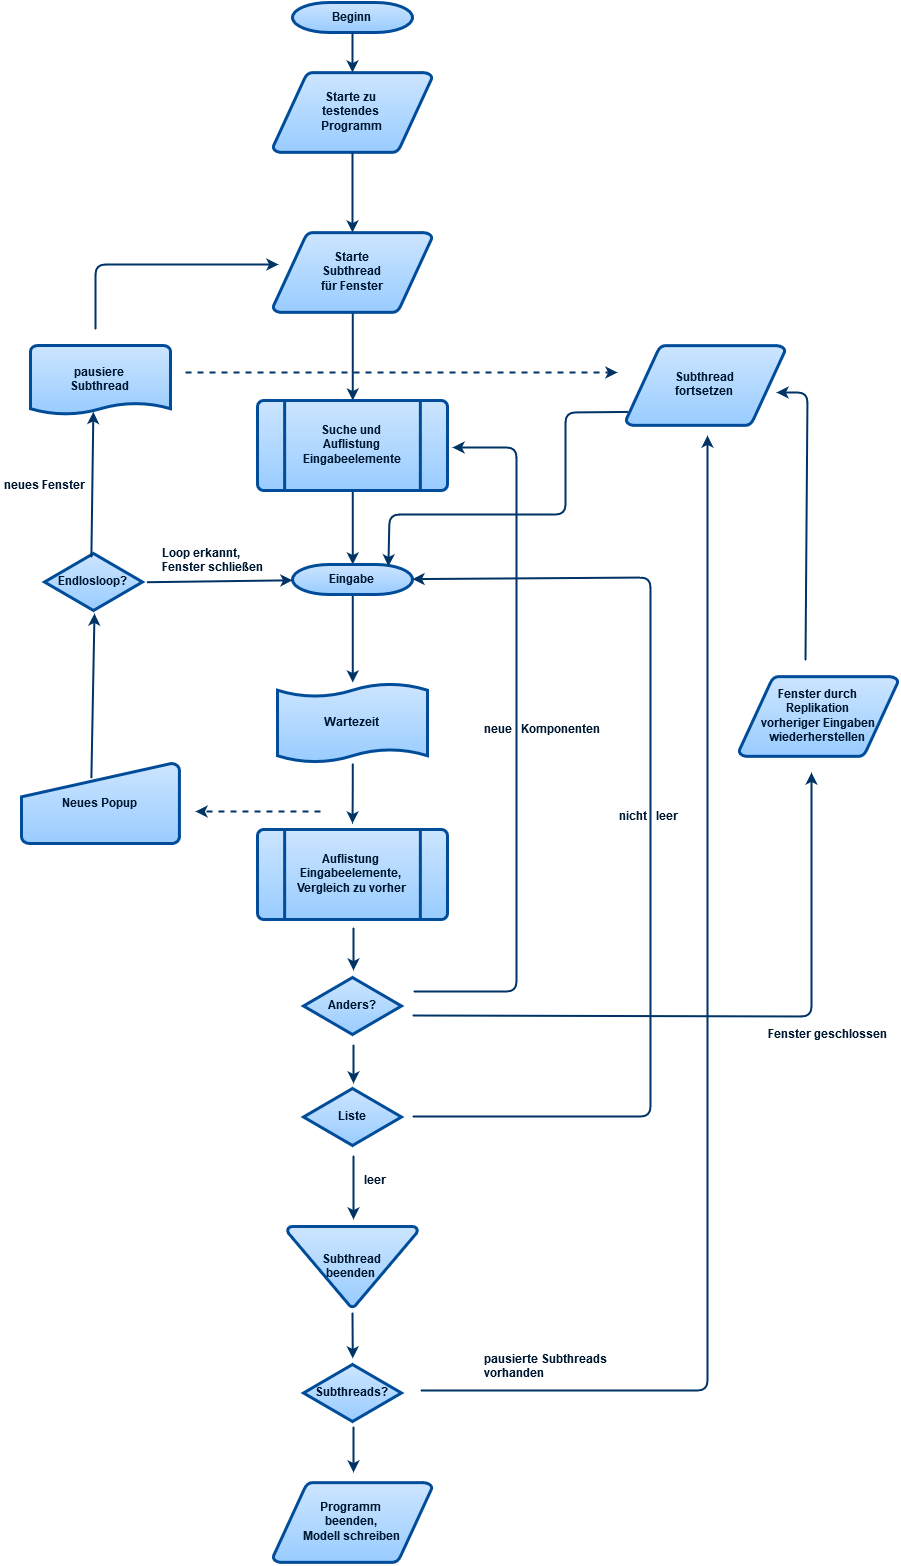
\includegraphics[width=0.85\textwidth]{bilder/autotester.png}
	\caption{Schematischer Ablauf des Autotesters}
	\label{fig:autotesterschematic}
\end{figure}

\begin{algorithm} \SetAlgoLined
	\KwData{Laufender Test $T$, neues Fenster/Popup $P$}
	\KwResult{Alle an $P$ anhängigen Komponenten wurden getestet, Test $T$ setzt fort}
	vorherige Testinstanz $T$ anhalten, sichert Zustand\;
	$Tn \longleftarrow Komponententester(P)$\;
	vorherige Testinstanz $T$ starten, Zustand wiederherstellen\;
	\caption{Popupbehandlung}
	\label{alg:autotesterpopup}
\end{algorithm}

\begin{algorithm} \SetAlgoLined
	\KwData{Wurzelkomponente/Fenster $A$, Liste von Problemstrings $StrL$;}
	\KwResult{Alle an $A$ anhängigen Komponenten wurden getestet}
	Komponentenliste $C: \longleftarrow A$ auf Komponenten durchsuchen\;
	$C$ ein Mal zufällig durchmischen\;
	\For{Komponente $k \in C$}
	{
		\If{$k \in Eingabeelemente$}
		{
			$k \longleftarrow \glqq{}Nutzereingabe\grqq{}$\;
			kurze Wartezeit (um GUI reagieren zu lassen)
		}
		\ElseIf{$k \in Texteingabeelemente$}
		{
			\For{String $s \in StrL$}
			{
				$k \longleftarrow \glqq{}Eintippen\grqq{} StrL$\;
				$k \longleftarrow \glqq{}Bestaetigung\grqq{}$\;
				sehr kurze Wartezeit (um GUI reagieren zu lassen)
			}
			$k \longleftarrow$ \glqq{}Eintippen\grqq{} zufälliges $s \in StrL$\;
		}
		\If{Auftreten neues Fenster/Popup $P$}
		{
			Popupbehandlung($P$)\;
		}
	}
	\caption{Komponententester}
	\label{alg:autotestermain}
\end{algorithm}

\begin{algorithm} \SetAlgoLined
	\KwData{Laufender Test $T$, vorheriger Test $Ta$, Fenster $F$ wurde vor Beendigung des Tests vom Programm geschlossen}
	\KwResult{Test $T$ setzt auf neuem, identischen Fenster $Fn$ fort}
	$Ts \longleftarrow$ laufende Testinstanz $T$ anhalten, sichert Zustand\;
	$T \longleftarrow Ta$, $T$ in Rückwärtslauf schalten\;
	\For{vorherige betätigte Komponente $k \in C(T)$}
	{
		\If{Auftreten Fenster $Fn$ mit $Fn == F$}
		{
			$T$ in Vorwärtslauf schalten\;
			Testinstanz $T$ wieder anhalten, sichert Zustand\;
			$T \longleftarrow Ts$, $F$ mit $Fn$ ersetzen, Zustand wiederherstellen\;
			Diese Suchschleife beenden, $T$ fortfahren lassen\;
		}
	}
	
	\caption{Verhalten bei Verlust des zu testenden Fensters}
	\label{alg:autotesterwindowloss}
\end{algorithm}


\subsection{Herausforderungen bei der Implementation}

Die Implementation des als Konzept vorliegenden Testers erfolgte iterativ
-- es war zu Beginn nicht sichergestellt, dass das Konzept als solches
überhaupt realistisch umsetzbar ist -- und passte sich während des
Entwicklungsprozesses laufend an neue Erkenntnisse und Erfahrungen
mit der Java-Swing-API und ihrem Verhalten an. Insbesondere
die asynchrone Eingabeverarbeitung und die resultierenden Probleme
bei der Verfolgung ihrer Auswirkungen waren eine technische Herausforderung.

Es traten häufig Situationen auf, in denen Ursache und Wirkung nicht
in Zusammenhang gebracht werden konnten. Der Prototyp beendete
Testabläufe vorzeitig oder geriet selbst in einen Fehlerzustand
oder fror ein. Unendliche Schleifen traten beim Testdurchlauf unregelmäßig auf.
Das ursprüngliche strikt deterministische Konzept wurde durch Zufallsdaten
erweitert, da es keine praktikable Alternative gibt, eine praktisch
unbegrenzte Zahl möglicher Schaltzustände zu testen -- gemeint
sind Eingabeelemente, die z.B. über einen AN/AUS Zustand verfügen,
oder eine einzelne Wahl zwischen mehreren Alternativen erfordern.
Fehler des Testers wurden durch die Fehlerabhandung des getesteten
Programms maskiert (und umgekehrt). Es musste ein Format gefunden
werden, durch das unbekannte beliebige Objekte bzw. Elemente aus den Daten
der graphischen Oberfläche für einen Menschen verständlich und prägnant
als Debug-Informationen in einer Konsole dargestellt werden können.

Dieses Format musste dann jeweils beim Auftreten neuer Elementarten
um den kleinsten gemeinsamen Nenner der zugrunde liegenden Klassen
erweitert werden. Für den Tester und damit eventuelle Nutzer von
Interesse sind nämlich nur die Daten, die ein graphisches Element
von seiner Funktion bzw. Bestimmung her von anderen unterscheidet.
Die übliche Implementation der Repräsentation als Zeichenkette
beinhaltet aber eine Anzahl überflüssiger oder irreführender
Informationen, wie z.B. die lokalen Koordinaten auf dem Bildschirm,
die absoluten und relativen Größenangaben der Fenster und ihrer
enthaltenen Elemente, oder nur für die kosmetische Darstellung
relevante Datenfelder.

Die laufende Änderung der sichtbaren graphischen Elemente als Reaktion
auf Eingaben war eine weitere Problematik, die es zu lösen galt.
Da nun ein Verfahren vorlag, um graphische Elemente miteinander
vergleichen zu können, konnte der gesamte an ein Element anhängige Baum
graphischer Elemente vor und nach Durchführung einer Eingabe ausgelesen
und die Ergebnisse miteinander verglichen werden. Es stellte sich heraus,
dass sowohl neue Elemente hinzukommen als auch bestehende Elemente im
Betrieb entfernt werden können. Dies muss vom Tester überwacht und
im Testablauf berücksichtigt werden. Neue zu Eingaben fähige Elemente werden 
an die Liste noch zu prüfender Eingabemöglichkeiten gehängt und
nicht mehr existierende Komponenten aus dieser Liste entfernt. Dies war
auch einer der Gründe für ein nichtdeterministisches Vorgehen:

Da Elemente nachträglich verschwinden können, also bei einem strikt
deterministischen Vorgehen nie getestet werden würden, kann nur ein
Verfahren mit Zufallselementen diese jemals erreichen. Die zufällige
Anordnung der Testreihenfolge stellt sicher, dass jedes durch Nutzung 
bzw. Eingaben in irgendeiner Reihenfolge erreichbares Element
irgendwann auch getestet wird. Dies unterstellt zwar eine unendliche
Anzahl an Testdurchläufen, aber für eine für alle praktischen Zwecke
unendliche Anzahl an möglichen Eingabekombinationen gibt es schlicht
keine Alternative. Auch sie hier erwähnt, dass ein menschlicher Tester
entschieden größere Schwierigkeiten damit hätte, wirklich zufällige
Eingabemuster umzusetzen -- Gewohnheiten beim Umgang mit Computern
und Eingabemasken verzerren das Testbild in Richtung eines eher
wahrscheinlichen Vorgangs, aber das Ziel des Konzepts ist ja gerade,
abseits dieser üblichen Pfade zu agieren.


\section{Problematische String-Eingaben}\label{section:naughtystrings}

Es wird eine online erhältliche, quelloffen gepflegte Liste aus Entwicklerkreisen verwendet, 
die \textbf{Big List of Naughty Strings} \footnote{\url{ https://github.com/minimaxir/big-list-of-naughty-strings }}. Diese enthält unter viele bekannte
Vertreter typischer Fehler oder Lücken bei der Verarbeitung von Zeichenketten in Programmen und
insbesondere auch im Internet. Es finden sich Zeichendarstellungen reservierter Begriffe wie
\glqq{}null\grqq{} oder \glqq{}true\grqq{}, SQL-Befehle, HTML und Javascript, exotische Unicode-Zeichen wie das
\glqq{}zero-width space\grqq{} \cite{unicodezerowidth} oder auch diverse DOS- oder Unix-spezifische
Anweisungen oder Optionen für Kommandozeilen.

Ziel ist es hierbei primär, mögliche durch Lücken in der Zeichenverarbeitung ausgelöste Probleme oder gar
Abstürze des Programms schnell herbeizuführen, damit diese diagnostiziert und behoben werden können.
Dies wird auch als \glqq{}Input Sanitization\grqq{} bzw. Eingabevalidierung bzw. -prüfung bezeichnet. 
Obwohl dieses Verfahren primär zur Verteidigung gegen Skript-Angriffe auf Webseiten dient
\footnote{\url{ http://www.scip.ch/?labs.20110914 }}, 
zählt eine wenig sinnvolle, aber dennoch mögliche Eingabe, 
die das zu testende Programm in der Ausführung beeinträchtigt oder sogar stoppt, klar zur 
Softwarequalität und sollte korrekt behandelt werden. Eine Fehlermeldung an den Nutzer zum
Beispiel ist eine völlig legitime Reaktion, eine unbehandelte Ausnahme dagegen nicht.

Je nach Betriebssystem führen unterschiedliche Symbole und Begriffe z.B. als Datei\-namen
manchmal zu sonderbaren Effekten und Fehlermeldungen oder sind schlicht verboten.
Beispiele hierfür wären \textbf{COM} oder auch von geschweiften Klammern \glqq{}\{\}\grqq{} umschlossene
Begriffe unter Windows, oder \textbf{dev} unter Linux. Programme, die ihre eigenen
Dateioperationen mit wählbaren Dateinamen durchführen, sehen häufig nicht eine vollständige
Behandlung all dieser möglichen Sonderfälle vor, und die Programmiersprache Java erzwingt
trotz vorgegebenen I/O-Ausnahme\-behandlungen nicht, alle Eventualitäten abzudecken.


\section{Zustandserfassung, -sicherung und -verfolgung sowie Kontrollmechanismen}\label{section:statemonitoring}

Um eine Überprüf-, Nachvollzieh- und Reproduzierbarkeit der vom automatischen Tester
durchgeführen Eingaben sicherzustellen, müssen diese bei jedem Testdurchlauf erschöpfend
mitprotokolliert werden. Da die Erstellung eines Modells der zu testenden Anwendung 
ebenfalls als Ziel definiert wurde, bietet sich ein Graph als Datenstruktur an. Die Analogie
eines solchen sowohl zum Java-AWT/Java-Swing-Datenmodell als auch zu den meisten 
Automatendarstellungen der Informatik lässt eine einfache und intuitive Implementation
erhoffen. Auch lassen sich die von einer Applikation geöffneten Fenster als Knoten und die
dorthin führenden Eingaben als Knotenübergänge auffassen, und es existieren
fertige Java-Bibliotheken für normierte Graphdarstellung. Für dieses Projekt genutzt
werden die quelloffene Graphbibliothek \textbf{JGraphT} \footnote{\url{ http://http://jgrapht.org/ }} sowie die
ebenfalls offene Visualisierungsplattform \textbf{Gephi} \footnote{\url{ http://gephi.github.io/ }}.

Sobald man die Frage nach dem \textbf{Wie} beantwortet hat, stellt sich als Nächstes
eine ähnliche nach dem \textbf{Was}. Unglücklicherweise sind Java-Applikationen der realen
Welt nicht nach akademischen Maßstäben gläsern und überschaubar. Kurz nach dem
Start eines konkreten Testdurchlaufs für \textbf{FirstSpirit} durch den Autotester zeigt der
Java-Debugger bereits 20 verschiedene Threads oder Kontrollfäden an, die alle auf
die eine oder andere Weise den Tester oder das Testobjekt beeinflussen können.
Java ist objektorientiert \cite{java7insel}, was im Gegensatz zu den Alternativen 
wie imperativen oder funktionellen Programmen in der Theorie erlaubt, jede laufende 
Instanz eines Programms in einen für Menschen verständlichen Datensatz zu übersetzen.

In der Praxis zeigt sich aber, dass die Masse an Kontrollfäden, Objekten und
sich gegenseitig beeinflussenden Nebeneffekten eine vollständige Zustandserfassung
und -verfolgung äußerst impraktikabel, wenn auch nicht völlig unmöglich, macht.
Das zu testende Programm muss folglich als \glqq{}Black Box\grqq{} verstanden werden.
Obwohl wir technisch in der Lage sind, die Inhalte einzusehen, ist die genaue
Funktion ein Rätsel, und wir können lediglich Rückschlüsse aus beobachtetem
Verhalten ziehen. Für unsere Zustandserfassung heißt dies, dass wir lediglich
die Klasse einer dargestellten Oberflächenelements sowie aus globalen
Schnittstellen erhältliche Informationen nutzen können, um einen beliebigen Zustand
von einem anderen zu unterscheiden. 

Diese Methodik hängt bis zu einem gewissen Grad von der jeweiligen Implementation 
des getesteten Programms ab und ist nicht frei von möglicher Ambivalenz,
insbesondere bei generellen, häufig benutzten Elementen -- wenn aber
das Verhalten eines Objekts von Instruktionen und nicht von Daten abhängt,
gibt es für den Tester keine praktikable Möglichkeit, dies festzustellen
oder ohne Kontext irgendetwas sinnvolles mit der Information anzufangen.

Ein Beispiel hierfür ist im Rahmen des FirstSpirit-Programms die Klasse
\glqq{}SearchDialog\grqq{}. Sie dient der Auswahl einer Datei oder eines Verzeichnisses
des Betriebssystems. Die Klasse beinhaltet keine Datenfelder, die für
eine Identifizierung einer konkreten Instanz hilfreich wären. Sie ist
Unterklasse von \glqq{}SelfDisposingDialog\grqq{}, welches ebenfalls keine Felder
enthält, und schließlich \glqq{}JDialog\grqq{}, eine Basisklasse der Java-Swing-API.
Diese garantiert nun die Präsenz eines Titels für jedwede Instanz
seiner Klassen, selbst wenn dieser nicht definiert oder leer sein sollte.
Worin unterscheiden sich nun verschiedene Instanzen von \glqq{}SearchDialog\grqq{}?

Die Antwort ist leider: In den Anweisungen, die an die Schnittstellen
des jeweiligen Objekts geschrieben wurden. Wir können dazu auf einen
aussagekräftigen, eindeutigen Titel des Suchfensters hoffen. Die
Anweisungen lesen und vergleichen zu wollen wäre zwar theoretisch
möglich, aber praktisch nutzlos. Die Instanz ist von Ihrem Nutzungskontext
abhängig, und Kontext ist etwas, dass der Autotester nicht verstehen kann.
Lediglich die Eingaben, die zu dem Suchfenster geführt haben,
lassen weitere Rückschlüsse darauf zu, wofür es dienen könnte.

Für den Autotester und eine für Menschen verständliche Protokollierung
wurde die Lösung einer eigenen \textbf{toString()} Methode gewählt.
Hierbei nimmt der Tester ein beliebiges darstellbares Objekt aus dem Testprogramm,
vergleicht es mit einer Reihe von der Java-Swing-API vorgegebenen
Objekten und Schnittstellen, und wählt eine passende Textdarstellung aus.
Üblicherweise ist dies der \glqq{}simple Classname\grqq{}, der einfache Klassenname,
da dieser nach gängigen Java-Konventionen den Nutzen einer Klasse zumindest
andeutet, kombiniert mit den möglicherweise vorhandenen kritischen Daten
der spezifischen Typklasse. Im Falle eines Fensters beispielsweise wäre
dies die Zeichenkette, die in der Titelzeile angezeigt wird. Im Fall
eines beschrifteten Knopfes die Beschriftung. Im Fall eines Knopfs
nur mit Glyphe oder Icon, ohne jegliche Beschriftung, 
ziehen wir den \glqq{}Tooltip\grqq{} bzw. Nutzungshinweis heran,
die vom Programmierer vorgesehene helfende Zeichenkette, die angezeigt
wird, wenn der Nutzer seinen Mauszeiger kurz über das betreffende Symbol hält.
Wir verlassen uns also auf gängige Programmierpraxis sowie Eigenarten der 
Java-Datenstrukturen, um ähnliche Instanzen zu identifizieren.

Zur Verfolgung des Programmzustands kann entsprechend nur die Liste
bzw. das Protokoll vergangener Eingaben an Elemente der Oberfläche
herangezogen werden. Um einen bestimmten Zustand zu reproduzieren,
ist die einzig sichere Lösung, alle dahin führenden Schritte nachzuahmen.
Es ist zwar häufig möglich, auch auf einem direkteren Weg zu einer
vermuteten Fehlerstelle zu gelangen, aber es muss immer damit gerechnet
werden, dass ein bestimmter Fehler nur bei perfekter Reproduktion
einer gewissen Eingabekette auftritt. 

Die Schwierigkeit beim
Verfolgen des Zustands der Java Virtual Machine verhindert
gleichzeitig auch das Einfrieren oder Abspeichern eines bestimmten Zustandes
zwecks späterer Wiederherstellung. Java sieht überhaupt nicht vor,
den gesamten Systemzustand sichern und laden zu können. Eine dennoch
denkbare Möglichkeit ist die Verkapselung des Testsystems in einer
virtuellen Umgebung, die beliebig pausiert, gespeichert und geladen
werden kann. Dies ist aber enorm aufwändig und würde zumindest eine
Kommunikation zwischen virtuellem System (bzw. einer Kontrolleinheit
ausserhalb desselben) und des darin laufenden Tests erfordern.
Auch ist der Speicher- und Ladevorgang selbst nicht unaufwändig,
da ein komplettes modernes Betriebssystem als Speicherabbild zumindest einige hundert
Megabyte an Informationen umfasst.

Virtualisierung ist dennoch ein guter Ansatz, um die Tests
durchzuführen. Da der Ablauf selbst nichtdeterministisch ist,
spricht nichts dagegen, eine Vielzahl von Testinstanzen parallel ablaufen zu
lassen. Man muss nur beachten, dass zu viele parallele Instanzen den VM-Host
so stark belasten können, dass die vom Tester eingelegten Pausen
zwischen Eingaben nicht mehr ausreichen könnten, um die jeweilige graphische
Oberfläche reagieren zu lassen. Dies würde eine korrekte Verfolgung
der aus Eingaben erfolgten Reaktionen zumindest sehr schwierig,
wahrscheinlich sogar unmöglich machen.


\subsection{Repräsentation der Programmzustände als Graph}

Eine eigene Graphimplementation für das Projekt zu verfassen wäre
außerhalb des Rahmens, daher wurde nach einem möglichst verbreitetem
Datenstandard und passenden Bibliotheken gesucht. Die Wahl fiel auf
die quelloffenen Projekte der Graphbibliothek \textbf{JGraphT} \footnote{\url{ http://http://jgrapht.org/ }} 
sowie der Visualisierungsplattform \textbf{Gephi} \footnote{\url{ http://gephi.github.io/ }}.
Das gewählte Datenformat ist \textbf{.graphml} \footnote{\url{ http://graphml.graphdrawing.org/specification.html }}.
Es handelt sich hierbei um einfache Textdateien im \textbf{xml}-Format,
welche auch menschlich noch lesbar und verständlich sind, und notfalls
auch editiert oder korrigiert werden könnten. 

Innerhalb des Testers erstellt JGraphT während des Testvorgangs 
ein Datenmodell des Graphen der getesteten Applikation. Nach erfolgreichem
Abschluss desselben wird das Resultat in besagtem graphml-Format
in einer eindeutig nach dem Testdatum benannten Datei abgespeichert.
Diese Datei ist dann zwar vollständig und auch von Menschen lesbar,
aber noch absolut undurchsichtig. Visualisierung ist notwendig,
um die Informationen in eine verständliche Form zu bringen.
Hierzu wird wahlweise Gephi verwendet. Es öffnet graphml-Dateien
und erlaubt die automatische Neuanordnung eines Graphen auf dem
Bildschirm, um maximale Ansehnlichkeit zu erzielen.

Nach einigen Probeläufen erwies sich der in Gephi mitgelieferte 
Yifan-Hu-Algorithmus \cite{hu2005efficient} als gut geeignet,
um einen komplexen Graph sternförmig auszubreiten. Ein beispielhaftes
Ergebnis lässt sich auf Seite \pageref{fig:model_firstspirit_notext}
begutachten. In der Grundeinstellung werden die von GraphT
abgespeicherten Knotendaten bzw. Programmzustände nicht angezeigt.
Diese relativ umfangreichen Zeichenketten erfordern für eine minimale
Lesbarkeit noch manuelles Verschieben und Sortieren der Graphknoten.
Ist dies aber erfolgt, erhält man aus dem Durchlauf eines blind testenden
Programms aber tatsächlich eine deckende Abbildung der getesteten
Applikation bzw. Ihrer möglichen Fensterdarstellungen. Zu sehen
ist ein solches finales Resultat auf Seite \pageref{fig:model_freespirit_06.10.2015}.

Einige Anmerkungen zu diesen Bildern: Der Knotensortieralgorithmus
nimmt auf die in diesem Fall ungewöhnlich langen Beschriftungen der einzelnen
Knoten keine Rücksicht. Für eine irgendwie lesbare Darstellung müssen die
Graphen nach der automatischen Sortierung noch per Hand verschoben werden,
bis keine Texte mehr überlappen. Ein weiteres Zugeständnis an Lesbarkeit
ist die Darstellung von Eingaben bzw. betätigter Schaltflächen als
Knoten. Eigentlich sollten Knoten nur Zustände darstellen, Eingaben
sind die Kanten bzw. Übergänge zwischen Zuständen. Dies führt aber dazu,
dass die langen Texte der Eingabedarstellungen an den Kanten dargestellt
werden, die nicht beliebig verschoben werden können. Sie liegen immer
zwischen zwei Knoten. Eine vernünftige Darstellung in dieser Form
erwies sich als unmöglich. Wenn die Eingaben ebenfalls als Knoten
dargestellt werden, können sie in der Darstellung beliebig verschoben
werden, sodass auch ihre Texte nicht überlappen und tatsächlich
gelesen werden können.


\section{Minimale Nichtautomatische Angaben}

Das Ziel eines vollautomatischen Tests kann leider nur annähernd erreicht werden,
wenn gleichzeitig andere Anforderungen wie \glqq{}Die Testzeit ist nicht unendlich lang\grqq{}
in Betracht gezogen werden müssen. Um auch die gewünschte graphische Oberfläche zu
testen und einige Fallstricke zu vermeiden, bietet der Autotester eine Konfigurationsdatei
nach dem Java \glqq{}Properties\grqq{} Standard, in der einige Angaben gemacht werden können bzw. müssen:

\begin{itemize}
  \item \textsc{targetGUISimpleClassName} der Klassenname der zu testenden Oberfläche
  \item \textsc{testStartDelayInSeconds} eine kurze Pause nach dem Start der Oberfläche, um Ladezeiten zuzulassen
  \item \textsc{blackListedAbstractButtons} nach dem Benennungs-Prinzip des Autotesters definierte unantastbare Standard-Schaltflächen
  \item \textsc{blackListedWindowKeywords} nach dem Benennungs-Prinzip des Autotesters definierte ignorierte Fenster
  \item \textsc{blackListedComponentsSimpleClassNames} nach Java-Klassenbezeichnungen definierte unantastbare Eingabeelement-Klassen
  \item \textsc{blackListedComponentsByUtilString} nach dem Benennungs-Prinzip des Autotesters definierte unantastbare Eingabeelement-Klassen
  \item \textsc{sleepTimeMillisTextfieldEntries} Dauer der Wartezeit zwischen Texteingaben
  \item \textsc{sleepTimeMillisBetweenFakeMouseClicks} Dauer der Wartezeit zwischen Mauseingaben
  \item \textsc{modelOutputFolder} Absoluter Ordnerpfad im Dateisystem, in dem die Resultate gespeichert werden sollen
\end{itemize}

Diese Angaben genügen, um für das sehr komplexe FirstSpirit-Programm einen regelmäßig annähernd
vollständigen Testdurchlauf über alle existierenden Schaltflächen zu ermöglichen.
Die gewählte Zeit vor dem Testbeginn sind zehn Sekunden. FirstSpirit ist eine sehr umfangreiche,
vernetzte Applikation. Als unantastbare Schaltflächen definiert wurden der globale Knopf
zum Beenden von FirstSpirit, ein Knopf, der zum Start eines externen Internetbrowsers führt
(nicht Bestandteil des Tests), der Knopf, der in Standard-Dateiauswahlfenstern das Erstellen eines neuen
Ordners ermöglicht (wäre als Standard-Ausnahme vermutlich sogar sinnvoller), sowie drei
Debug-Schaltflächen, die die Logdatei des Testablaufs mit den Ausgaben des Programms selbst
überschwemmen können.

Als einziges ignoriertes Fenster wurde die \glqq{}FirstSpirit Zwischenablage\grqq{} definiert. Durch eine
Eigenart in der Implementation sind die resultierenden Fenster technisch gesehen immer neuartige
Instanzen, was zu einem unendlichen Test führt, da der Tester alle Fenster testen will.
Eine unendliche Anzahl von Fenstern führt leider auch zu einer unendlichen Anzahl an Tests.
Aus Effizienzgründen wurden als nächstes zwei häufig auftretende Klassen von Tests ausgeschlossen,
welche zwar technisch gesehen Eingaben erlauben, aber im FirstSpirit-Programm lediglich
darstellende Funktion haben. Dabei handelt es sich um \glqq{}GlowLabel\grqq{} und \glqq{}SynthScrollBarUI\grqq{}.
Für die eingestellten Pausen zwischen Text- und Mauseingaben haben sich zehn und 2000 Millisekunden
als geeignet herausgestellt. Dies hängt aber stark vom System ab, auf dem der Test durchgeführt wird,
und insbesondere der Auslastung des Systems. Wenn von einer virtualisierten Umgebung ausgegangen
wird, von der viele Instanzen parallel ablaufen, wäre es vermutlich sehr sinnvoll, diese
Pausen erheblich länger andauern zu lassen.

Zusätzlich zu diesen wenigen Angaben muss natürlich das Testprogramm auch in der Lage sein,
die zu testende Oberfläche als Unterprozess zu starten. Nur so kann der notwendige Zugriff
auf die Daten der laufenden Applikation erfolgen. Würde man zunächst das zu testende
Programm starten, und dann den Tester, wären beide in verschiedenen JVM-Instanzen
verkapselt, die jeweils keinen Zugriff aufeinander zulassen. Für einen solchen
Start als Unterprozess ist die Startklasse der zu testenden Applikation notwendig,
diese kann aus den Metainformationen einer lauffähigen Java \glqq{}JAR\grqq{}
ausgelesen werden. Zusätzlich bieten sich verschiedene Parameter bzw. Argumente
für die JVM an, die z.B. zusätzliche Speicherallokation oder einen anderen
Algorithmus für den Garbage Collector erlauben. Auch ist es bei gewissen Anwendungen,
darunter FirstSpirit, möglich, direkt im Programmstart Parameter wie Login-Daten
oder Programmports zu spezifizieren, um eine Testblockierende Login-Maske
zu überspringen.

Alternativ hätte ein System vorgesehen werden können, welches gewisse Eingaben
bei einem definierten Eingabefeld vorschreibt. Dies wäre für maximale Kompatibilität
hilfreich, wenn ein Programm solche Kommandozeilen-Parameter nicht zulässt.
In diesem Fall hat es sich aber als unnötig erwiesen. Es sei auch die
Annahme in den Raum gestellt, dass nur Entwickler diese Testapplikation
verwenden werden, also in jedem Fall Zugriff auf Quellcode besteht,
und ein entsprechendes Feature relativ schnell und einfach an bestehende
Applikationen angefügt werden kann. Wenn nicht -- der Autotester selbst
wird vermutlich quelloffen verfügbar sein, und eine Implementation
dieser Idee kann von interessierten Parteien umgesetzt werden.


\subsection{\glqq{}minimale\grqq{} Angaben in der Praxis}

In der weitergehenden Nutzung des Autotesters mit verschiedenen
Programmen wurde klar, dass eine gewisse Anpassungs- oder
Lernzeit des Programms mit dem Testsubjekt zwingend notwendig ist.
Über die Definition des Anwendungsfensters hinaus müssen für
effiziente Durchläufe in jedem Fall die Schaltflächen, die Beendigung
des jeweiligen Programms resultieren, auf die Blacklists gesetzt
werden. Darüber hinaus hat jedes getestete Programm eine oder
mehrere Eingaben oder Fenster, die in einem unendlichen oder
sonst unbrauchbaren Durchlauf resultierten -- es wäre vermutlich
eine gute Idee, den Tester um eine maximale Laufzeit oder
eine maximale Prüftiefe oder etwas Ähnliches zu erweitern.

Auch müssen eventuelle Abstürze des getesteten Programms
abgefangen oder verhindert werden. Unerwartetes Beenden
der Abwendung macht die gewonnenen Erkenntnisse abseits
der Konsole unbrauchbar, da eigentlich auf einen
vollständigen Graphen sowie eine Logdateie hin gearbeitet wurde.
Eine Methodik, die auch Logdateien von unerwartet beendeten
Durchläufen sichert, wäre sinnvoll. In der Praxis läuft
die Nutzung der Autotesters nun so ab, dass ein Entwickler
zunächst die Startklassen und Umgebungsvariablen einrichtet
sowie das Anwendungsfenster der zu testenden Applikation
angibt. Der Autotester leistet hierbei Unterstützung, er
gibt die für ihn sichtbaren Anwendungsfenster an. Anschließend
lässt der Entwickler den Autotester laufen, bis sich die Anwendung
selbst beendet oder unerwartet beendet wird, liest die Logdatei
um den Grund bzw. die ausschlaggebende Eingabe zu ermitteln,
und setzt evtl. ein Fenster oder eine Komponente auf die
Blacklist in der Konfigurationsdatei. Er passt gleichzeitig
die Wartezeiten zwischen den Eingaben an die allgemeine
Verarbeitungsgeschwindigkeit der Anwendung auf dem jeweiligen
Computer an. Je nach Anwendung sind hier nun viele oder
sehr wenige Angaben nötig, um konsistent volle Durchläufe
zu ermöglichen. FirstSpirit hat neun Einträge
in seiner Konfigurationsdatei, jEdit und yEd haben beide
acht. Tendenziell sind allerdings bei yEd die meisten Eingaben
und Fenster vom Test ausgeschlossen, da zwischenzeitlich
partielle Angaben für den Ausschluß implementiert und auch
direkt genutzt wurden.
